\documentclass[conference]{IEEEtran}
\IEEEoverridecommandlockouts
% The preceding line is only needed to identify funding in the first footnote. If that is unneeded, please comment it out.
\usepackage[noadjust]{cite}
\usepackage{amsmath,amssymb,amsfonts}
\usepackage{algorithmic}
\usepackage{graphicx}
\usepackage{textcomp}
\usepackage{xcolor}

\def\BibTeX{{\rm B\kern-.05em{\sc i\kern-.025em b}\kern-.08em
    T\kern-.1667em\lower.7ex\hbox{E}\kern-.125emX}}
\begin{document}

\title{Peningkatan Kinerja Modul Pencocokan Pola dalam Sistem Deteksi Intrusi Snort Menggunakan GPU\\
{\footnotesize \textsuperscript{*}Note: Sub-titles are not captured in Xplore and
should not be used}
\thanks{Identify applicable funding agency here. If none, delete this.}
}

\author{
\IEEEauthorblockN{Afrizal Fikri}
\IEEEauthorblockA{{School of Electrical Engineering and Informatics} \\
{Institut Teknologi Bandung}\\
{Bandung, Indonesia} \\
afrizalf96@gmail.com}
\and
\IEEEauthorblockN{Achmad Imam Kistijantoro}
\IEEEauthorblockA{{School of Electrical Engineering and Informatics} \\
{Institut Teknologi Bandung}\\
{Bandung, Indonesia} \\
imam@informatika.org}
}

\maketitle

\begin{abstract}
    % The advancement of technology has been giving contributions to the rapid growth of the use of digital data. In this digital era, lots of physical data have been transformed into the digital ones. One example of the use of digital data is the digital biometric fingerprint data on the Electronic Identity Card (KTPel). Fingerprint matching can take a long time to process if the data is large enough. Thus, there is a need for a parallel fingerprint matching.  Based on this rationale, this paper aims to improve the fingerprint matching performance, in the current state of the art linear solution, by using the Minutia Cylinder-Code (MCC) algorithm in parallel on GPU. Based on the experiment and testing, the proposed solution has a significantly better run time compared to the state of the art linear solution while maintaining the accuracy. 

    The advancement of technology has been giving contributions to the rapid growth of the use of digital data. In this digital era, lots of physical data have been transformed into the digital ones. Among those, a lot of confidential data also take place. Thus, security assurance become important as well. One of the entry point of those malicious usages come from server side. Ensuring authority on server utilizing network intrusion detection system (NIDS) could take enormous resource and time. One of the important part of NIDS is string matching part inside the analyzer. Based on this rationale, this paper aims to improve matching speed of detection in order to maximize overall system throughput using GPU instead of CPU. Based on the experiment and testing, the proposed solution has a significantly better run time compared to the state of the art linear solution while maintaining the accuracy. 
\end{abstract}

\begin{IEEEkeywords}
    pattern matching; intrusion detection; GPU; parallel computation; CUDA
\end{IEEEkeywords}

\section{Introduction}
This document is a model and instructions for \LaTeX.
Please observe the conference page limits. 

\section{String Matching}
In general, there are two kinds of string matching: single pattern string matching and multi pattern string matching. We will focus into multi pattern string matching. There are several famous algorithms for multi pattern string matching: Aho-Corasick, Commentz-Walter, and Wu-Manber algorithm. This paper will try to implement variation of Aho-Corasick algorithm.

    \subsection{Aho-Corasick Algorithm}
    Aho-Corasick algorithm is kind of string matching algorithm works by matching one string to a dictionary. This dictionary contains all pattern to be matched in form state machine. 
    
    In this algorithm, matching operation is performed by traversing state machine by characters in input string. If any of the final state reached, then input string matched one of the patterns. Matching continued until input string is terminated. 

    \begin{figure}[htbp]
        \centerline{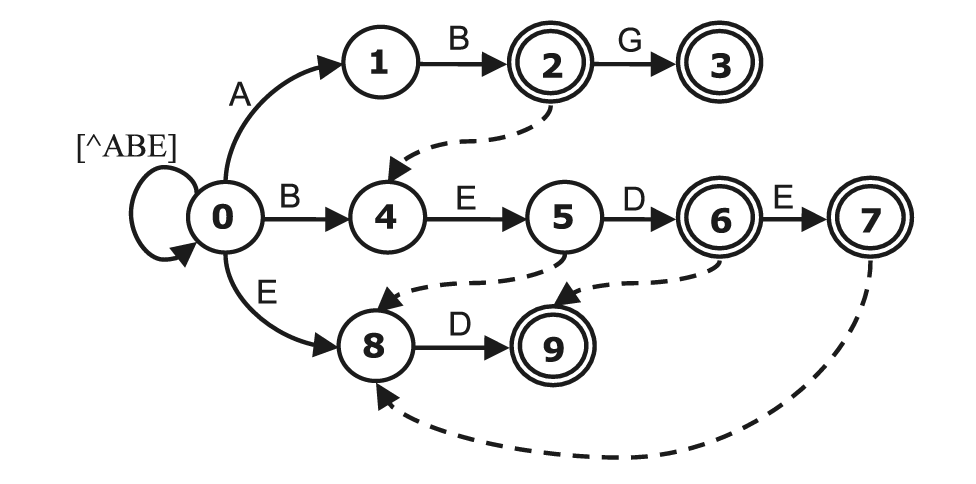
\includegraphics[width=0.4\textwidth]{../src/resources/aho-c.png}}
        \caption{Example state machine of Aho-Corasick dictionary.}
        \label{fig}
    \end{figure}

    Aho-Corasick use failure function to perform backtrack after stop at one of the final states. Failure function will redirect this final state to longest pattern prefix which match suffix of the currently matched pattern. Failure function reduce the need of repeating another same sequence which just matched by. By this method, all of containing patterns can be matched by one pass and reducing complexity from $O(mn)$ to $O(n)$. 

    In this algorithm, memory lookup become bottleneck. Every traversal operation will fetch one entry from table. Since memory accesses are more expensive than computations, this algorithm is memory bound.

    \subsection{Data Parallel Aho-Corasick}
    In order to extend Aho-Corasick into multithreading, we need to divide the load of matching for each threads. One of the method is by partitioning input into several chunks and then each threads will match this sequence into dictionary. But as we encounter a pattern span multiple chunks at once, it is not recognized on either threads. This problem known as boundary detection problem. So, we need to extend matching by length of the longest pattern. Memory lookup thus increase to $O((n/s + m) * s) = O(n + ms)$ for $s$ is amount of chunks. 

    \begin{figure}[htbp]
        \centerline{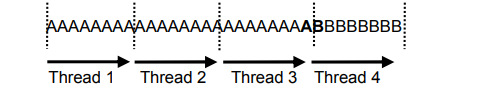
\includegraphics[width=0.4\textwidth]{../src/resources/boundary.png}}
        \caption{Pattern \textbf{AB} not recognized by both thread 3 and 4}
        \label{fig}
    \end{figure}

    \subsection{Parallel Failureless Aho-Corasick}
    Another method to adapt multithreading Aho-Corasick is to spread threads to all characters byte. Each threads will matching any pattern begin with each coresponding character and terminate if any of final state or no valid transition occurs \cite{lin2013}. The consequence is eavery character will match only one pattern at most.
    Thus, no need to make any failure function. And also boundary detection problem will not occur by using this approach.

    \begin{figure}[htbp]
        \centerline{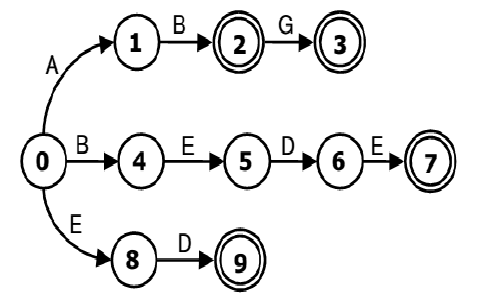
\includegraphics[width=0.4\textwidth]{../src/resources/pfac.png}}
        \caption{State machine without failure function}
        \label{fig}
    \end{figure} 

\section{Related Works}

    \subsection{Utilization of Double Buffering Scheme, Texture Memory and Pinned Memory}

        In this paper, GPU-based matching implementation had been proposed using Aho-Corasick algorithm. Beside utilization of GPU multithreading, there are few adjustment to import Aho-Corasick to GPGPU. State machine built using transition table on 2D table on texture memory. Based on experiment, this implementation improving performance by 19\% \cite{gnort2008}.
        For the memory transfer scheme, double buffering scheme was proposed. Packets will be batched in one buffer. Whenever the buffer gets full, all packets are transferred to the GPU in one operation. Transfer from device to host also done in same way. All result will be batched in the second buffer and get transferred when gets full.
        Another optimization trick used is using pinned memory. Both of the buffer in host will be pinned to reduce swappiness. And pinned memory also enable DMA transfer and reducing computation needs and latency. This design can improve system performance until 3.2 times higher than implementation using multithreading on CPU.

    \subsection{Maximizing GPU Utilization by Pipelining}

        % Sehingga dalam penelitian ini, diajukan beberapa optimasi untuk pencocokan \emph{rule option}. Salah satu optimasi yang diajukan untuk tahap pencocokan yaitu penggunaan \emph{pipelining}. \emph{Pipelining} dilakukan dengan memisahkan \emph{thread} yang digunakan untuk operasi \emph{I/O} dengan operasi analisis. Kemudian pada tiap operasi \emph{I/O}, akan dilakukan pengumpulan paket dalam \emph{batch} sebelum dilakukan transfer antar komponen. Implementasi dilakukan dengan menggunakan basis IDS Snort.

        % Pengujian dilakukan dengan konfigurasi CPU ganda Intel X5680 dengan 12 core dan dua GPU NVIDIA GTX 580. Hasil yang didapatkan menggunakan desain ini mampu mencapai 1,5 sampai 4 kali lipat kinerja Snort. \emph{Latency} dapat menurun hingga 13 mikrodetik pada \emph{offloading} paket awal untuk batch sebesar 1,5 kB. Pada pengujian dengan \emph{traffic} jaringan, rancangan ini mampu mencapai \emph{throughput} 25,2 Gbps pada \emph{input} sebesar 40 Gbps.

        By profiling, it is concluded that bottleneck occured on 3 components: packet acquisition, multi pattern string matching, and option rule matching by regular expression. Moreover, inside string matching component alone, 

    \subsection{Failureless Aho-Corasick by Maximizing Shared Memory Usage}

        Salah-satu algoritma yang sering digunakan dalam deteksi pola adalah Aho-Corasick yang bersifat \emph{multi-pattern string matching}. Dalam penelitian yang dilakukan \cite{lin2013}, dilakukan optimasi pada implementasi algoritma Aho-Corasick pada GPU. Implementasi memanfaatkan fitur-fitur pada GPU seperti \emph{memory coalescing}, penghematan transaksi pada \emph{global memory}, dan akses \emph{shared memory} yang bebas \emph{bank-conflict}.

        Desain akan menggunakan pendekatan algoritma AC tanpa \emph{failure function} yaitu PFAC (\emph{Parallel Failureless Aho-Corasick}). Pendekatan ini dapat memaksimalkan penggunaan \emph{thread} pada GPU tanpa menyebabkan \emph{overlapping}. Transaksi ke \emph{global memory} dapat dikurangi dengan memuat transisi \emph{state} kosong ke \emph{shared memory} dan penggunaan \emph{texture memory} yang memanfaatkan \emph{cache}.

        Hasil pengujian dengan CPU Intel Core i7-950 dan GPU NVIDIA GTX 580 menunjukkan peningkatan yang signifikan. Optimasi dengan PFAC pada \emph{multithread} CPU mencapai 7 kali lipat dari AC. Sedangkan PFAC pada GPU dapat mencapai 10 kali lipat daripada AC pada CPU. Masukan didapatkan dari dataset \emph{traffic} kompetisi DEFCON.

\section{Proposed Solution}
    \subsection{Matching Algorithm}
    \subsection{State Machine Implementation}
    \subsection{\emph{Thread} Allocation}
    \subsection{GPU Optimation}

    % \begin{table}[htbp]
    % \caption{Table Type Styles}
    % \begin{center}
    % \begin{tabular}{|c|c|c|c|}
    % \hline
    % \textbf{Table}&\multicolumn{3}{|c|}{\textbf{Table Column Head}} \\
    % \cline{2-4} 
    % \textbf{Head} & \textbf{\textit{Table column subhead}}& \textbf{\textit{Subhead}}& \textbf{\textit{Subhead}} \\
    % \hline
    % copy& More table copy$^{\mathrm{a}}$& &  \\
    % \hline
    % \multicolumn{4}{l}{$^{\mathrm{a}}$Sample of a Table footnote.}
    % \end{tabular}
    % \label{tab1}
    % \end{center}
    % \end{table}

    % \begin{figure}[htbp]
    % \centerline{\includegraphics{fig1.png}}
    % \caption{Example of a figure caption.}
    % \label{fig}
    % \end{figure}

\section*{Acknowledgment}

The preferred spelling of the word ``acknowledgment'' in America is without 
an ``e'' after the ``g''. Avoid the stilted expression ``one of us (R. B. 
G.) thanks $\ldots$''. Instead, try ``R. B. G. thanks$\ldots$''. Put sponsor 
acknowledgments in the unnumbered footnote on the first page.

\bibliography{references}
\bibliographystyle{IEEEtran}

\end{document}
